\section{Evaluasi Model}

Model dilatih sesuai dengan konfigurasi yang telah disebutkan pada subbab \ref{sec:pelatihan-model} dan dilatih pada lingkungan eksperimen yang telah disebutkan pada subbab \ref{sec:lingkungan-eksperimen}. Eksperimen dilakukan pada setiap tugas evaluasi yaitu \nlptask. Setiap tugas evaluasi dilatih dengan \textit{fine-tuning}, \methodPEFT. Hasil evaluasi dilakukan pada 5-\textit{fold} dengan setiap evaluasi terdapat nilai rata-rata, minimum, dan maksimum dari \textit{fold} tersebut.

\subsection{Evaluasi Parameter Model}

Perhitungan parameter pelatihan sudah dijelaskan sebelumnya pada subbab \ref{sec:peft}. Pada subbab ini akan dijelaskan lebih lanjut terkait perhitungan pada model telah dilakukan pelatihan. Hasil dari setiap parameter pelatihan untuk setiap model dapat dilihat pada \ref{table:param-model} yang didapatkan dari pustaka Adapters. Model yang digunakan adalah IndoBERT dan IndoT5, yang berarti kedua model tersebut berbasis BERT dan T5 pada masing-masing model terkait. BERT merupakan model \textit{encoder} dengan spesifikasi $d_{hidden} = 768$ dan $intermediate_{size} = 512$. Sedangkan, T5 merupakan model \textit{encoder decoder} dengan spesifikasi yang sama dengan BERT, namun $block$ pada model T5 karena arsitekturnya yang mempunyai $encoder$ dan juga $decoder$. Pada subsubbab berikutnya, dilakukan perhitungan paramater pelatihan dan dibandignkan dengan hasil yang didapatkan pada tabel \ref{table:param-model}.

\begin{table}[h]
    \centering
    \caption{Parameter model IndoBERT dan IndoT5}
    \label{table:param-model}
    \resizebox{\textwidth}{!}{
        \begin{tabular}{l|lc|lc}
            \toprule
            \multirow{2}{*}{\textbf{Metode}} & \multicolumn{2}{c|}{\textbf{IndoBERT}} & \multicolumn{2}{c}{\textbf{IndoT5}} \\
            & \textbf{\#Parameter} & \textbf{\%Parameter} & \textbf{\#Parameter} & \textbf{\%Parameter} \\
            \midrule
            \textit{Fine-tuning} & 110M & 100\% & 223M & 100\% \\
            LoRA ($r$=8) & 0.294M & 0.268\% & 0.885M & 0.397\% \\
            LoRA ($r$=16) & 0.590M & 0.536\% & 1.769M & 0.794\% \\
            Prefix Tuning ($pl$=5) & 9.853M & 8.912\% & 29.560M & 13.261\% \\
            Prefix Tuning ($pl$=50) & 9.887M & 8.943\% & 29.663M & 13.308\% \\
            Adapter ($rf$=64) & 0.231M & 0.209\% & 0.461M & 0.207\% \\
            Adapter ($rf$=16) & 0.895M & 0.809\% & 1.789M & 0.803\% \\
            UniPELT & 11.083M & 10.025\% & 32.346M & 14.511\% \\
            \bottomrule
        \end{tabular}
    }
\end{table}

\subsubsection{Perbandingan Parameter Model untuk Metode \textit{Adapter}}

Berdasarkan \textit{hyperparameter} untuk metode PEFT pada tabel \ref{table:hyperparameter-PEFT}, nilai dari $rf$ yang berarti $reduction\_factor$ adalah 16 dan 64. Sehingga, bisa didapatkan bahwa $d_{bottleneck}=48$ untuk $rf=16$ dan $d_{bottleneck}=12$ untuk $rf=64$. Dilakukan perhitungan untuk model IndoBERT dan IndoT5 pada $rf=16$, sedangkan $rf=64$ tidak akan dituliskan perhitungannya. Rumus yang digunakan untuk perhitungan adalah rumus \ref{eq:parameter-adapter}.

\begin{equation}
    \begin{aligned}
        block = 12 \\ 
        forward\_head = 1 \\
        W_{down} = W_{up} = 768 \times 48 \\
        W_{down} = W_{up} = 36.864 \\
        \psi_{IndoBERT(A)} = (36.884 + 48 + 36.884 + 768) \times 12 \times 1 \\
        \psi_{IndoBERT(A)} = 894.528 \\
    \end{aligned}
    \label{eq:calc-param-adapter-bert}
\end{equation}

Pada rumus \ref{eq:calc-param-adapter-bert}, didapatkan bahwa paramater dari model IndoBERT dengan metode \textit{Adapter} dengan $rf=16$ adalah 894.528 yang sesuai dengan tabel \ref{table:param-model}. Lalu, perhitungan yang sama dilakukan terhadap \textit{Adapter} dengan $rf=64$. Sehingga, didapatkan hasil untuk model IndoBERT pada $rf=16$ adalah 230.544 yang juga sesuai dengan \ref{table:param-model}. 

\begin{equation}
    \begin{aligned}
        block = 12 \\ 
        forward\_head = 2 \\
        W_{down} = W_{up} = 768 \times 48 \\
        W_{down} = W_{up} = 36.864 \\
        \psi_{A(IndoT5)} = (36.884 + 48 + 36.884 + 768) \times 12 \times 2 \\
        \psi_{A(IndoT5)} = 1.789.056 \\
    \end{aligned}
    \label{eq:calc-param-adapter-t5}
\end{equation}

Dari Rumus \ref{eq:calc-param-adapter-t5} didapatkan bahwa parameter dari model IndoT5 dengan metode \textit{Adapter} dengan $rf=64$ adalah 1.789.056 yang konsisten dengan tabel \ref{table:param-model}. Nilai $attention\_head$ pada model IndoT5 adalah 2 yang merupakan 2 kali dari $attention\_head$ pada IndoBERT karena IndoT5 merupakan \textit{encoder decoder}. \textit{adapter} ditambahkan setelah \textit{feed-forward}, dengan \textit{encoder decoder}, berarti terdapat 2 kali \textit{feed-forward} pada setiap \textit{layer}. Untuk $rf=64$ didapatkan hasil 461.088 yang juga konsisten. Semua hasil parameter konsisten jauh lebih kecil dibanding dengan \textit{fine-tuning} dengan hanya menggunakan sekitar 0.2\% sampai 0.8\%.

\subsubsection{Perbandingan Parameter Model untuk Metode \textit{Prefix-Tuning}}

Berdasarkan \textit{hyperparameter} untuk metode PEFT pada tabel \ref{table:hyperparameter-PEFT}, nilai dari $pl$ yang berarti $prefix_length$ adalah 5 dan 50. Perhitungan dilakukan untuk model IndoBERT dan IndoT5 pada $pl=5$. Sedangkan, untuk $pl=50$ tidak akan dituliskan perhitungannya. Rumus yang digunakan pada perhitungan ini adalah rumus \ref{eq:parameter-prefix-tuning}.

\begin{equation}
    \begin{aligned}
        block = 12 \\
        attention\_head = 1 \\
        Embedding_{IndoBERT} = 5 \times 768 \\
        Embedding_{IndoBERT} = 3.840 \\
        Linear1 = 768 \times 512 + 512 \\
        Linear1 = 393.728 \\
        Linear2 = (512 \times 768 + 768) \times 2 \times 24 \\
        Linear2 = 9.455.616 \\
        \psi_{IndoBERT(P)} = (3.840 + 393.728 + 9.455.616) \times 1 \\
        \psi_{IndoBERT(P)} = 9.853.184 \\
    \end{aligned}
    \label{eq:calc-param-pt-bert}
\end{equation}

Rumus \ref{eq:calc-param-pt-bert} mendapatkan hasil parameter dari model IndoBERT dengan metode \textit{Prefix-Tuning} $pl=5$ adalah 9.853.184 yang konsisten dengan tabel \ref{table:param-model}. Perhitungan yang sama dilakukan untuk $pl=50$ dengan mengganti nilai $Embedding_{IndoBERT}$ menjadi $50 \times 768$, didapatkan nilai parameternya adalah 9.887.744 yang konsisten juga.

\begin{equation}
    \begin{aligned}
        attention\_head = 3 \\
        block = 12 \times 2 \\
        Embedding_{IndoT5} = 5 \times 768 \\
        Embedding_{IndoT5} = 3.840 \\
        Linear1 = 768 \times 512 + 512 \\
        Linear1 = 393.728 \\
        Linear2 = (512 \times 768 + 768) \times 2 \times 24 \\
        Linear2 = 9.455.616 \\
        \psi_{IndoT5(P)} = (3.840 + 393.728 + 9.455.616) \times 3 \\
        \psi_{IndoT5(P)} = 29.559.552 \\
    \end{aligned}
    \label{eq:calc-param-pt-t5}
\end{equation}

Rumus \ref{eq:calc-param-pt-t5} mendapatkan hasil parameter dari model IndoT5 dengan metode \textit{Prefix-Tuning} $pl=5$ adalah 29.559.552 yang sesuai dengan tabel \ref{table:param-model}. Nilai $attention\_head$ pada model T5 adalah sebanyak 3, sama dengan arsitektur \textit{transformer} dengan 1 $attention\_head$ pada \textit{encoder} dan 2 $attention\_head$ pada \textit{decoder}. Perhitungan juga dilakukan untuk $pl=50$ didapatkan nilai parameternya 29.633.232 yang juga konsisten. Hasil untuk semua parameter pelatihan pada metode \textit{Prefix-Tuning} konsisten lebih kecil dibanding \textit{fine-tuning} dengan menggunakan sekitar 9\% sampai 13\% parameter.


\subsubsection{Perbandingan Parameter Model untuk Metode LoRA}

Berdasarkan \textit{hyperparameter} untuk metode PEFT pada tabel \ref{table:hyperparameter-PEFT}, nilai dari $r$ yang berarti $rank$ adalah 8 dan 16. Perhitungan dilakukan untuk model IndoBERT dan IndoT5 pada $r=8$. Sedangkan, untuk $r=16$ tidak akan dituliskan perhitungannya. Rumus yang digunakan pada perhitungan ini adalah rumus \ref{eq:parameter-lora}.

\begin{equation}
    \begin{aligned}
        attention\_head = 1 \\
        block = 12 \\
        \psi_{IndoBERT(L)} = ((2 \times 768 \times 8) \times 2 \times 12) \\
        \psi_{IndoBERT(L)} = 294.912
    \end{aligned}
    \label{eq:calc-param-lora-bert}
\end{equation}

Rumus \ref{eq:calc-param-lora-bert} mendapatkan hasil parameter pelatihan dari model IndoBERT dengan metode LoRA $r=8$ adalah 294.912 yang konsisten dengan hasil yang didapatkan pada tabel \ref{table:param-model}. Perhitungan yang sama dilakukan pada rumus \ref{eq:calc-param-lora-bert} dengan mengganti nilai $r$ menjadi 16, didapatkan hasil yaitu 589.824 yang juga konsisten.

\begin{equation}
    \begin{aligned}
        attention\_head = 3 \\
        block = 12 \\
        \psi_{IndoT5(L)} = ((2 \times 768 \times 8) \times 2 \times 12) \times 3 \\
        \psi_{IndoT5(L)} = 884.736
    \end{aligned}
    \label{eq:calc-param-lora-t5}
\end{equation}

Didapatkan hasil dari rumus \ref{eq:calc-param-lora-t5} untuk model IndoT5 dengan metode LoRA $r=8$ adalah 884.736 yang konsisten dengan hasil pada \ref{table:param-model}. Nilai $attention\_head$ pada model T5 adalah 3 kali dibanding model IndoBERT karena modelnya \textit{encoder decoder}. Perhitungan yang sama dilakukan dengan nilai $r=16$, didapatkan hasil 1.769.472 yang konsisten dengan tabel \ref{table:param-model}. Metode LoRA mendapatkan hasil yang konsisten jauh lebih kecil dengan hanya menggunakan sekitar 0.3\% sampai 0.8\% parameter saja.

\subsubsection{Perbandingan Parameter Model untuk Metode UniPELT}

Metode UniPELT tidak mempunyai konfigurasi yang bisa dimodifikasi. Konfigurasi untuk setiap metode PEFT pada UniPELT adalah \textit{Adapter} $rf=16$, \textit{Prefix-Tuning} $pl=10$, dan LoRA $r=8$. Semua metode PEFT tersebut sudah didapatkan perhitungannya pada subsubbab sebelumnya, kecuali untuk \textit{Prefix-Tuning} $pl=10$. Sehingga, dilakukan perhitungan dengan rumus \ref{eq:parameter-prefix-tuning} yang mengasilkan rumus \ref{eq:cacl-param-pt-pl10}.

\begin{equation}
    \begin{aligned}
        \psi_{IndoBERT(P)} = 9.857.024 \\
        \psi_{IndoT5(P)} = 29.571.072 \\
    \end{aligned}
    \label{eq:cacl-param-pt-pl10}
\end{equation}

Selanjutnya, dilakukan perhitungan pada model IndoBET dan IndoT5 untuk metode UniPELT dengan rumus \ref{eq:parameter-unipelt}. Dengan didapatkan rumus \ref{eq:cacl-param-pt-pl10}, perhitungan bisa dilakukan seperti yang bisa dilihat pada rumus \ref{eq:cacl-param-unipelt-bert}. Model BERT mempunyai 1 $attention\_head$ dan juga 1 $forward\_head$ yang berasal dari 1 \textit{encoder}. Didapatkan hasil parameter pelatihan yaitu 11.083.376 yang sesuai dengan tabel \ref{table:param-model}.

\begin{equation}
    \begin{aligned}
        block = 12 \\
        attention\_head = 1 \\
        forward\_head = 1 \\
        gating = 768 \times 1 + 1 \\
        gating = 769 \\
        total\_gating = (3 \times 1 + 1) \times 769 \times 12 \\
        total\_gating = 36.912 \\
        \psi_{IndoBERT(U)} = 894.528 + 9.857.024 + 294.912 + 36.912 \\
        \psi_{IndoBERT(U)} = 11.083.376
    \end{aligned}
    \label{eq:cacl-param-unipelt-bert}
\end{equation}

Perhitungan juga dilakukan untuk model IndoT5. Model T5 mempunyai 3 $attention\_head$ dan 2 $forward\_head$ yang berasal dari arsitektur \textit{encoder decoder}. Dari rumus \ref{eq:cacl-param-unipelt-t5}, didapatkan hasil parameter pelatihan yaitu 32.346.372 yang sesuai dengan tabel \ref{table:param-model}. Hasil parameter pelatihan model pada UniPELT konsisten dengan semua metode PEFT sebelumnya. Selain itu, jika dibandingkan dengan \textit{fine-tuning}, metode UniPELT konsisten dengan parameter yang lebih kecil dengan sekitar 10\% samapi 15\% parameter.

\begin{equation}
    \begin{aligned}
        block = 12 \\
        attention\_head = 3 \\
        forward\_head = 2 \\
        gating = 768 \times 1 + 1 \\
        gating = 769 \\
        total\_gating = (3 \times 3 + 2) \times 769 \times 12 \\
        total\_gating =  101.508 \\
        \psi_{IndoT5(U)} = 1.789.056 + 29.571.072 + 884.736 + 101.508 \\
        \psi_{IndoT5(U)} = 32.346.372 \\
    \end{aligned}
    \label{eq:cacl-param-unipelt-t5}
\end{equation}

\subsection{Hasil Evaluasi NER}

\begin{figure}[h]
    \centering
    \centerline{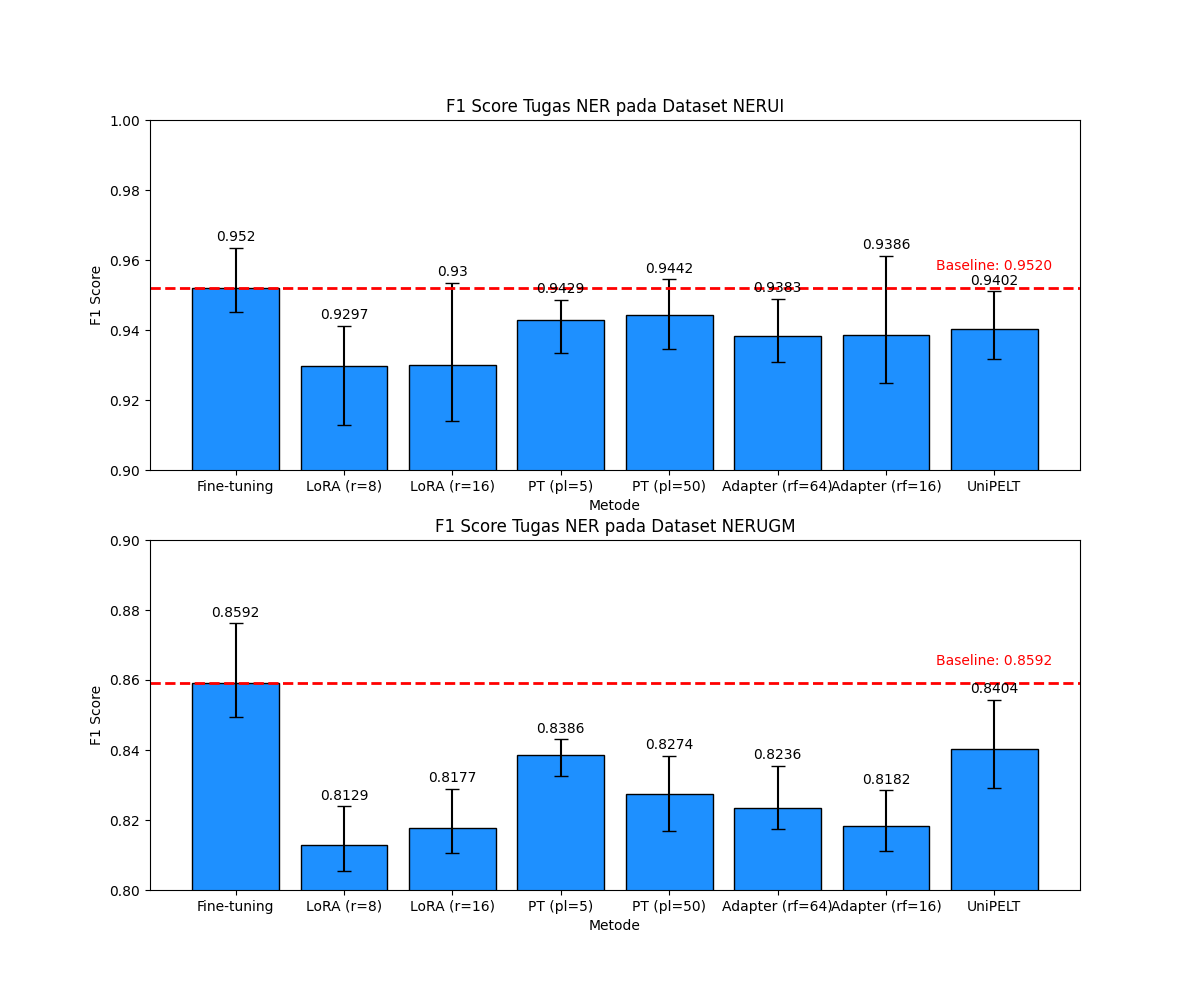
\includegraphics[width=1.2\textwidth]{chapter-4/ner_result.png}}
    \caption{\textit{F1 Score} Hasil Evaluasi NER}
    \label{fig:ner-result}
\end{figure}

\begin{table}[h]
    \centering
    \caption{Waktu pelatihan tugas NER}
    \label{table:runtime-ner}
    \resizebox{\textwidth}{!}
    {
        \begin{tabular}{l|cc|cc}
            \toprule
            \multirow{2}{*}{\textbf{Metode}} & \multicolumn{2}{c|}{\textbf{NER UI}} & \multicolumn{2}{c}{\textbf{NER UGM}} \\
            & \textbf{Waktu(s)} & \textbf{\%Peningkatan} & \textbf{Waktu(s)} & \textbf{\%Peningkatan} \\
            \midrule
            \textit{Fine-tuning} & 884 & 0\% & 974 & 0\% \\
            LoRA ($r$=8) & 528 & 40\% & 580 & 40\% \\
            LoRA ($r$=16) & 515 & 42\% & 588 & 40\% \\
            Prefix Tuning ($pl$=5) & 494 & 44\% & 562 & 42\% \\
            Prefix Tuning ($pl$=50) & 534 & 40\% & 598 & 39\% \\
            Adapter ($rf$=64) & 564 & 36\% & 587 & 40\% \\
            Adapter ($rf$=16) & 563 & 36\% & 595 & 39\% \\
            UniPELT & 928 & -5\% & 991 & -2\% \\
            \bottomrule
        \end{tabular}
    }
\end{table}

\subsection{Hasil Evaluasi \textit{Sentiment Analysis}}

\begin{figure}[h]
    \centering
    \centerline{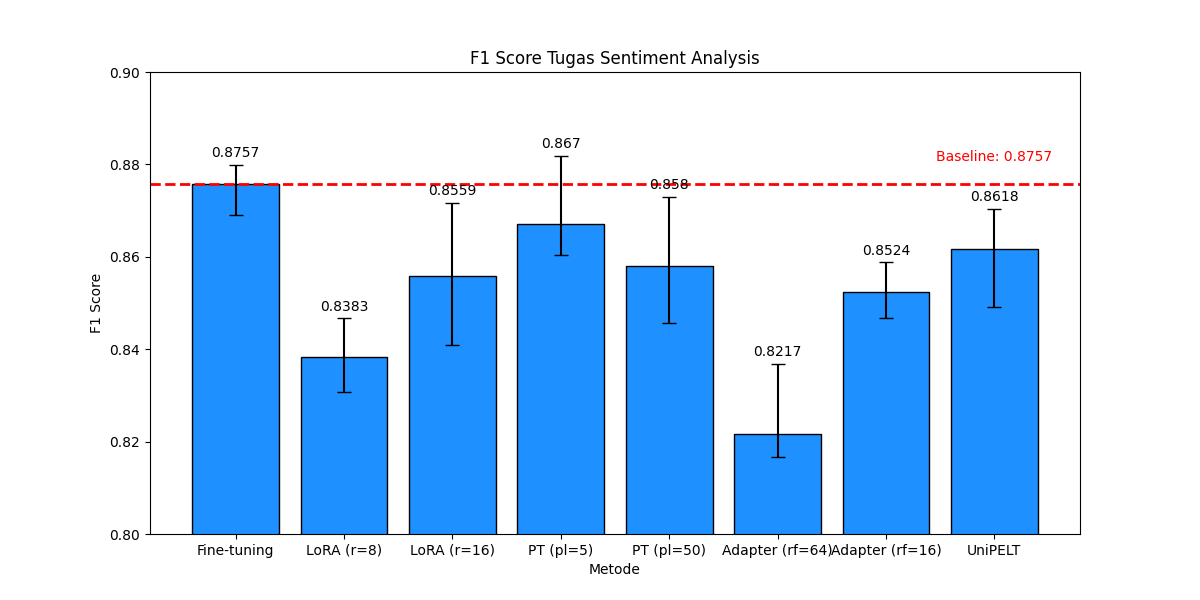
\includegraphics[width=1.2\textwidth]{chapter-4/sentiment_result.png}}
    \caption{\textit{F1 Score} Hasil Evaluasi \textit{Sentiment Analysis}}
    \label{fig:sentiment-result}
\end{figure}

\begin{table}[h]
    \centering
    \caption{Waktu pelatihan tugas \textit{sentiment analysis}}
    \label{table:runtime-sentiment}
    \begin{tabular}{l|cc}
        \toprule
        \textbf{Metode} & \textbf{Waktu(s)} & \textbf{\%Peningkatan} \\
        \midrule
        \textit{Fine-tuning} & 866 & 0\% \\
        LoRA ($r$=8) & 627 & 28\% \\
        LoRA ($r$=16) & 627 & 28\% \\
        Prefix Tuning ($pl$=5) & 619 & 28\% \\
        Prefix Tuning ($pl$=50) & 652 & 25\% \\
        Adapter ($rf$=64) & 613 & 29\% \\
        Adapter ($rf$=16) & 617 & 29\% \\
        UniPELT & 746 & 14\% \\
        \bottomrule
    \end{tabular}
\end{table}

\subsection{Hasil Evaluasi \textit{Summarization}}

\begin{figure}[h]
    \centering
    \centerline{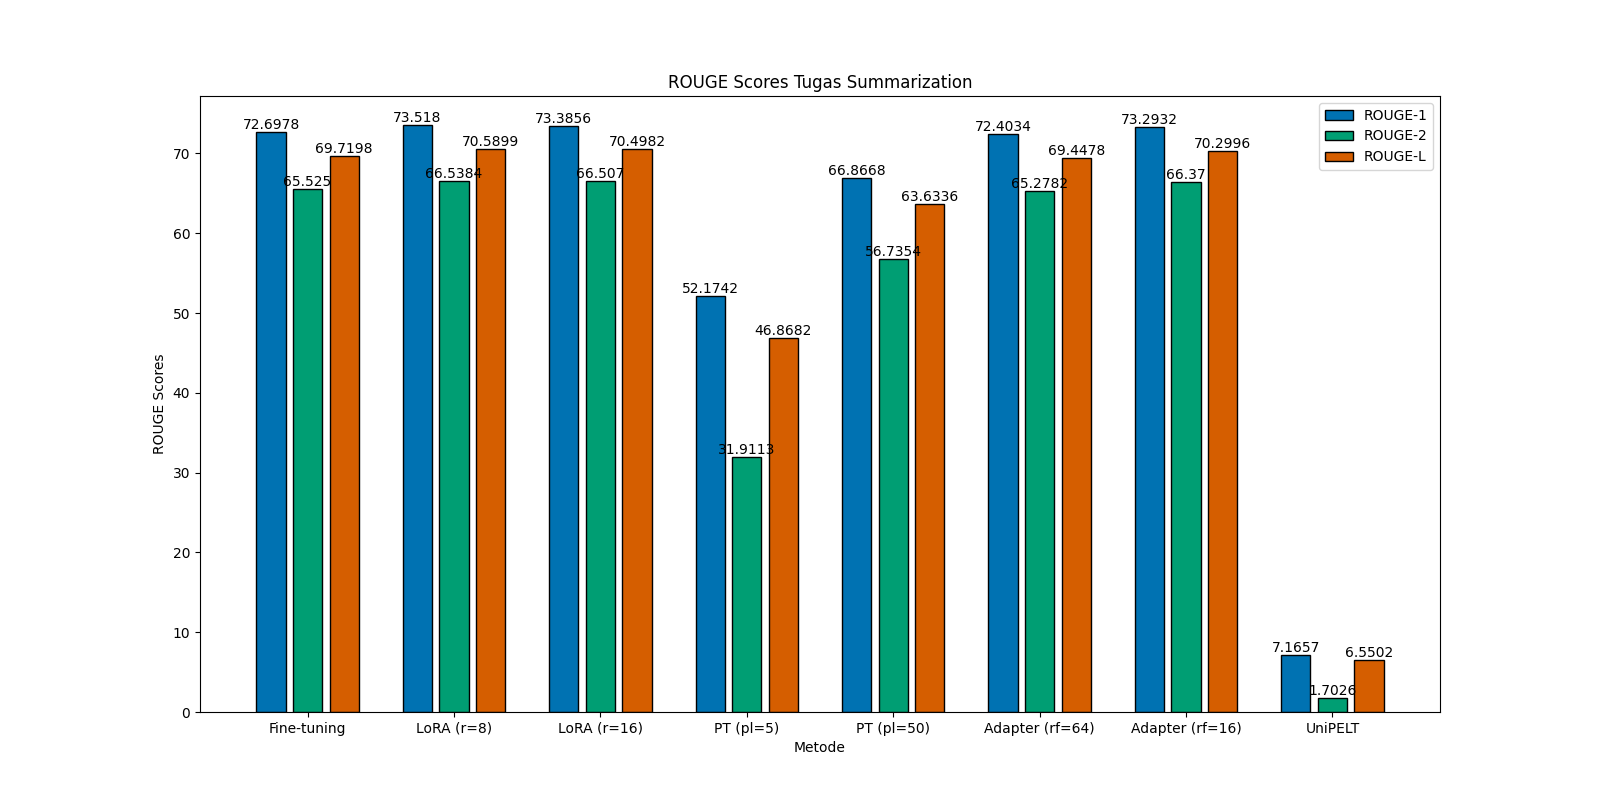
\includegraphics[width=1.4\textwidth]{chapter-4/summarization_result.png}}
    \caption{ROUGE \textit{Score} Hasil Evaluasi \textit{Summarization}}
    \label{fig:summarization-result}
\end{figure}

\begin{table}[h]
    \centering
    \caption{Waktu pelatihan tugas \textit{summarization}}
    \label{table:runtime-summarization}
    \begin{tabular}{l|cc}
        \toprule
        \textbf{Metode} & \textbf{Waktu(s)} & \textbf{\%Peningkatan} \\
        \midrule
        \textit{Fine-tuning} & 5026 & 0\% \\
        LoRA ($r$=8) & 4841 & 4\% \\
        LoRA ($r$=16) & 4900 & 3\% \\
        Prefix Tuning ($pl$=5) & 6618 & -32\% \\
        Prefix Tuning ($pl$=50) & 11379 & -127\% \\
        Adapter ($factor$=64) & 4578 & 9\% \\
        Adapter ($factor$=16) & 4587 & 9\% \\
        UniPELT & 9241 & -84\% \\
        \bottomrule
    \end{tabular}
\end{table}
